\documentclass[10pt, a4paper]{article}
\usepackage[utf8]{inputenc}
\usepackage{amsmath}
\usepackage{amssymb}
\usepackage{amsthm}
\usepackage{parskip}
\usepackage{enumitem}
\usepackage{siunitx}
\usepackage{tikz}
\usepackage{pgfplots}
\usepackage{graphicx}
\graphicspath{ {./} }
\usetikzlibrary{arrows.meta}
\usetikzlibrary{angles,quotes}
\pgfplotsset{compat = newest}

\title{Física Contemporánea\\Resolución de Tarea 2}
\author{Vite Riveros Carlos Emilio\\ Romero De La Rosa Gabriela Michelle\\ 
        Fisher Bautista Emir Julián\\ López Gallegos Fátima}
\date{18 octubre del 2022}

\begin{document}
    \maketitle

    \begin{enumerate}
        \item Problemas
        \begin{enumerate}
            \item Un cuerpo esta apoyado sobre un plano inclinado de coeficiente de rozamiento
            estático $\mu_c$. El ángulo de inclinación del plano se incrementa hasta alcanzar un
            ángulo crítico $\alpha_{c'}$, después del cual el cuerpo comienza a deslizar. ¿Cuál es el
            coeficiente de rozamiento $\mu_e$.

            \begin{center}
                Se tiene que si $\alpha\leq\alpha_c$, entonces la masa $m$ está en reposo. A su vez, la 
                fuerza de fricción máxima que se puede obtener antes de que el objeto comience a acelerar
                es $|y_{\text{max}}|=|\mu_e N|$. Observandoel diagrama de fuerzas y dado que el objeto
                está en reposo hasta $\alpha_e$ se tiene que:

                $F_x= ma_x= 0= W_x - |\gamma|$, $F_y=ma_y=0=|N|-W_y$

                Notemos que $W_x=W\sin\alpha=mg\sin\alpha$, $W_y=W\cos\alpha=mg\cos\alpha$, $|F|=\mu_e|N|$
                y dado que $W_y-|\gamma|=0$ y $|N|=W_y=mg\cos\alpha$, se tiene que $|\gamma|=\mu_e|N|=\mu_e mg\cos\alpha$.

                Por lo tanto, $mg\sin\alpha-\mu_e mg\cos\alpha=0$, de donde $mg\sin\alpha=\mu_e mg\cos\alpha$.
                Es decir $\mu_e\cos\alpha=\sin\alpha$, entonces $\mu_e=\frac{\sin\alpha}{\cos\alpha}=\tan\alpha$
                si $\alpha\leq\alpha_c$, o séase $\mu_e=\tan\alpha_c$

            \end{center}

            \item Dos niños son arrastrados por un trineo sobre un terreno cubierto de nieve.
            El trineo es jalado por una cuerda que forma un ángulo de 40 grados con la
            horizontal. La masa conjunta de los dos niños es de 45 kilos y el trineo tiene
            una masa de 5 kilos. Los coeficientes de rozamiento estático y cinemático son
            $\mu_e = 0.2$ y $\mu_c = 0.15$. Determinar la fuerza de rozamiento ejercida por el suelo
            sobre el trineo y la aceleración de los niños y el trineo si la tensión de la cuerda
            es $140\si{N}$.

            \begin{center}
                $F_x=ma_x=T_x-\gamma$\\
                $ma_x=107\si{N}-60\si{N}$\\
                $a_x\frac{47\si{N}}{50\si{Kg}}=0.94\frac{\si{m}}{\si{s^2}}$

                $Fr=60\si{N}$, $a_x=0.94\frac{\si{m}}{\si{s^2}}$
            \end{center}

            \begin{center}
                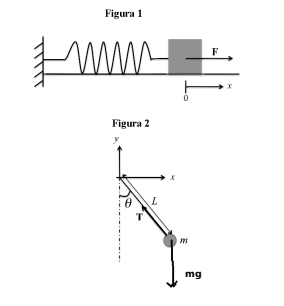
\includegraphics{image}
            \end{center}

            \item Considere el resorte de la figura 1 y suponga que en el extremo derecho se
            le aplica una fuerza en la dirección positiva del eje x de magnitud 6N, 9N,
            12N, 15N, y 18N, y que el estiramiento resultante del resorte bajo la acción
            de esta fuerza es de 1.0cm, 1.5cm, 2.0cm, 2.5cm y 3.0cm respectivamente. 1.
            Haga una gráfica de la fuerza aplicada en función de la longitud que se estiro
            el resorte en cada caso y diga si el resorte obedece la ley de Hooke. En caso
            afirmativo determine la constante del resorte k. 2. Suponga que el mismo resorte
            se suspende verticalmente del techo de una habitación y que del extremo libre
            se cuelga una masa m1 que provoca que el resorte se estire 2.7cm. Determine
            el valor de m1. 3. Discuta la validez de la ley Hooke si del mismo resorte se
            suspende una masa m2 = 100Kg.

            1.
            \begin{center}
                \begin{tikzpicture}[scale=.6]
                    \begin{axis}[
                        xlabel={$F$}, 
                        ylabel={$r$},
                        xmin=0, 
                        xmax=19, 
                        ymin=0, 
                        ymax=3.2,
                        xtick={6,9,12,15,18}, 
                        ytick={0,1,1.5,2,2.5,3}]
                        \addplot[mark=square]table
                        {
                            x   y
                            0   0
                            6   1
                            9   1.5
                            12  2
                            15  2.5
                            18  3
                        };
                    \end{axis}
            \end{tikzpicture}
            \end{center}
            
            El resorte obedece la ley de Hooke, ya que la relación entre la fuerza ejercida y la 
            distancia es una relación lineal. Y la constante $k$ se calcula de la siguiente manera:

            \begin{center}
                $F = kr$, $F=\{6N,9N,12N,15N,18N\}$, $r=\{1\si{cm},1.5\si{cm},2\si{cm},2.5\si{cm},3\si{cm}\}$\\
                $r=\{.01\si{m},.015\si{m},.02\si{m},.025\si{m},.03\si{m}\}$

                $k= \frac{F}{r}$\\

                $k= 600$

            \end{center}

            \begin{center}
                2. $F = kr$, $r=2.7\si{cm}=.027\si{m}$, $k = 6$\\
                $F = 600(.027)$\\
                $F=16.2\si{N}$\\
                $F=m_1g$, $g=9.83\si{\frac{m}{s^2}}$\\
                $16.2\si{N}=m_1(9.83\si{\frac{m}{s^2}})$\\
                $m_1=\frac{16.2\si{N}}{9.83\si{\frac{m}{s^2}}}$

                $m_1=1.648\si{kg}$
            \end{center}

            3. No creo que la ley de Hooke se mantenga para toda cantidad de masa, ya que al llegar a cierto grado de fuerza
            el resorte tendría que deformarse en la vida real. 

            \item Considere una partícula de masa $m$ suspendida de un hilo de longitud $L$ cuya
            masa es despreciable. El sistema descrito se ilustra en la figura 2 abajo y es
            conocido como péndulo simple. 1. Haga un diagrama del cuerpo libre para la
            masa $m$ y escriba las ecuaciones de movimiento en las direcciones $\hat\imath$ y $\hat\jmath$. 2.
            Escriba las coordenadas $x$ y $y$ en función del ángulo $\theta$ y la longitud del hilo $L$
            y obtenga la primera y segunda derivadas $\frac{d^2x}{dt^2}$ y $\frac{d^2x}{dt^2}$. Sustituya estas
            expresiones en las ecuaciones para las componentes de la fuerza del inciso 1. 3.
            Observe que multiplicando las últimas ecuaciones del inciso 2 por $\cos\theta$ y $\sin\theta$
            respectivamente es posible eliminar la tensión $T$. La ecuación resultante es la
            ecuación de movimiento del péndulo simple. 4. Compruebe que para ángulos
            pequeños la ecuación diferencial es la misma que la ley de Hooke. Ángulos
            pequeños significa que $\sin\theta$ se puede aproximar por $\theta$. Verifique que para $\theta \approx 15 \si{rad}$ 
            la aproximación es correcta.

            \begin{center}
                La única fuerza en el eje $x$ es $T_x=T\sin\theta$ pero dudo a que se oponga al movimiento de 
                la masa, se tiene que:\\
                $F_x=ma_x=-T\sin\theta$\\
                $a_x=-\frac{T}{m}\sin\theta$\\
                $\frac{d^2x}{dt^2}=-\frac{T}{m}\sin\theta$\\

                Mientras que en el eje $y$ se tiene:\\
                $F_y=ma_y=T\cos\theta-mg$\\
                $a_y=\frac{T}{m}\cos\theta-\si{g}$\\
                $\frac{d^2y}{dt^2}=\frac{T}{m}\cos\theta-\si{g}$

                La posición de la masa $m$ la podemos describir con $x=l\sin\theta$ y $y=-l\cos\theta$. 
                El signo negativo viene a que se encuentra por debajo de la horizontal. 

                Dado $x=l\sin\theta$\\
                $\frac{dx}{dt}=l\cos\theta\frac{d\theta}{dt}$\\
                $\frac{d^2x}{dt^2}=l(-\sin\theta(\frac{d\theta}{dt})^2+\cos\theta\frac{d^2\theta}{dt^2})$


                Dada $y=-l\cos\theta$\\
                $\frac{dy}{dt}=l\sin\theta\frac{d\theta}{dt}$\\
                $\frac{d^2y}{dt}=l(\cos\theta(\frac{d\theta}{dt})^2+\sin\theta\frac{d^2\theta}{dt^2})$

                $\sin\theta(\frac{d\theta}{dt})^2= \cos\theta\frac{d^2\theta}{dt^2} + \frac{T}{ml}\sin\theta$\\
                $\cos\theta\sin\theta(\frac{d\theta}{dt})^2=\cos^2\theta\frac{d^2\theta}{dt^2}+\frac{T}{ml}\cos\theta\sin\theta$\\
                $\cos\theta(\frac{d\theta}{dt})^2=\frac{T}{ml}\cos\theta-\frac{\si{g}}{l}-\sin\theta\frac{d^2\theta}{dt^2}$\\
                $\cos\theta\sin\theta(\frac{d\theta}{dt})^2=\frac{T}{ml}\cos\theta\sin\theta-\frac{\si{g}}{l}\sin\theta-\sin^2\theta\frac{d^2\theta}{dt^2}$

                $\cos^2\theta\frac{d^2\theta}{dt^2}+\frac{T}{ml}\cos\theta\sin\theta=\frac{T}{ml}\cos\theta\sin\theta-\frac{\si{g}}{l}\sin\theta-\sin^2\theta\frac{d^2\theta}{dt^2}$\\
                $\frac{d^2\theta}{dt^2}=-\frac{\si{g}}{l}\sin\theta$

                Para ángulos pequeños, es posible aproximar $\sin\theta\approx\theta$. Por lo que se puede
                escribir como:

                $\frac{d^2\theta}{dt^2}=-\frac{\si{g}}{l}\theta$

                Para $x=\frac{\pi}{12}$:\\
                $\sin(\frac{\pi}{12})=0.2588$\\
                $\frac{\pi}{12}\approx 0.2617$\\
                $|\sin(\frac{\pi}{12})-\frac{\pi}{12}|\approx 0.00298$

                Podríamos establecer el límite de nuestra aproximación a $\frac{\pi}{12}$ radianes o $\ang{15}$.


            \end{center}

            \item Un bulto de $400 \si{Kg}$ de masa se eleva hasta una plataforma a una altura de $1.5 \si{m}$
            por medio de un plano inclinado de $6 \si{m}$ de longitud. Calcular la fuerza paralela
            al plano que es necesaria aplicar y el trabajo realizado, suponiendo que no existe
            rozamiento.

            \begin{center}
                $\alpha = \frac{1.5}{6}=\sin{.25}=\ang{14}$\\
                $F=mg(\sin\alpha)$\\
                $F=(400\si{Kg})(9.8\si{\frac{m}{s^2}})(\sin\ang{14})$\\
                $F=980\si{N}$\\
                $W=Fd$\\
                $W=(980\si{N})(6\si{m})=5880\si{J}$
            \end{center}

            \item Una fuerza $\vec{F} = ( 6\hat\imath - 2\hat\jmath )\si{N}$ actúa sobre una partícula que experimenta un
            desplazamiento $\vec{s} = ( 3\hat\imath + \hat\jmath )\si{m}$. Encuentre: 1. El trabajo realizado por la fuerza
            sobre la partícula. 2. El ángulo relativo entre $\vec{F}$ y $\vec{s}$.

            \begin{center}
                $\si{W} = \vec{F} \cdot \vec{r}$\\
                $\si{W} = (6\hat\imath - 2\hat\jmath) \cdot (3\hat\imath + \hat\jmath)$\\
                $\si{W} = (6\hat\imath(3\hat\imath)) + (-2\hat\jmath(1\hat\jmath))$\\
                $\si{W} = 6(3)+(-2)=18-2=16\si{J}$
            \end{center}

        \end{enumerate}

        \item Preguntas
        \begin{enumerate}
            \item Supón que te subes a dos básculas de piso con tu peso dividido por igual entre
            las básculas. ¿Cuál sera la lectura de cada báscula? ¿Qué sucede si apoyas más
            de tu peso sobre un pie y menos sobre el otro?

            \begin{center}
                La lectura de las básculas sería la mitad del peso, esto al estar posicionado todo en 
                dos puntos de apoyo. Sin embargo, al apoyar más un pie y menos el otro, la lectura se vería
                afectada, aumentando más en en la báscula donde apoyemos más el pie. Esto sería así
                debido a que nuestro punto principal de apoyo sería ese pie, y de esta forma, cargaría más
                con todo nuestro peso.
            \end{center}

            \item Considera las dos fuerzas que actúan sobre una persona que permance quieta;
            el tirón de la gravedad hacia abajo y el apoyo del piso hacia arriba. ¿Son estas
            fuerzas iguales y opuestas? ¿Forman un par de acción y reacción? ¿Por qué sí o
            por qué no?

            \begin{center}
                Si nos basamos en la tercer ley de Newton, en efecto, estas fuerzas serían iguales y opuestas.
                Serían un par de acción y reacción puesto que la acción sería el estar parado, con la gravedad
                jalando hacia el centro de la tierra, y la reacción es la fuerza que se ejerce y la misma que
                evita que nos hundamos en la tierra hasta llegar al núcleo.
            \end{center}

            \item Cuando una partícula gira en círculo, una fuerza central actúa sobre ella en
            dirección al centro de rotación. ¿Por qué esta fuerza no efectúa trabajo sobre la
            partícula?

            \begin{center}
                No efectúa el trabajo debido a que la dirección de la fuerza es radial y el desplazamiento
                es instantáneo, es tangencial, perpendicular a la trayectoria $w=Fd\cos\alpha$. El ángulo
                $\alpha$ entre el desplazamiento y la fuerza es $\ang{90}$ y $\cos\ang{90}=0$.
            \end{center}

            \item ¿Qué requiere mas trabajo: levantar un costal de 50 kg una distancia vertical de
            2 m o jalar 2 m en la horizontal el mismo costal?

            \begin{center}
                Sin duda alguna, levantar un costal de $50\si{Kg}$ a $2\si{m}$ de distancia vertical requiere
                mucho más esfuerzo que solo jalarlo $2\si{m}$ en horizontal. Esto mismo se debe a que, al levantarlo
                su peso caerá sobre nosotros, haciendo que se ejerza una mayor fuerza sobre nuestro cuerpo. Y si lo jalamos,
                la fuerza ejercida será sobre el suelo, permitiéndonos a nosotros movernos con mayor facilidad. 
            \end{center}

        \end{enumerate}
    \end{enumerate}
\end{document}
